\documentclass[12pt]{beamer}
\newenvironment{ConCodigo}[1]
  {\begin{frame}[fragile,environment=ConCodigo]{#1}}
  {\end{frame}}
\graphicspath{{Imagenes/}{../Imagenes/}}
\usepackage[utf8]{inputenc}
\usepackage[spanish]{babel}
\usepackage{hyperref}
\usepackage{etex}
\reserveinserts{28}
\usepackage{amsmath}
\usepackage{amsthm}
\usepackage{mathtools}
\usepackage{multicol}
\usepackage{multirow}
\usepackage{tabulary}
%\usepackage{tabularx}
\usepackage{booktabs}
\usepackage{nccmath}
\usepackage{biblatex}
\usepackage{epstopdf}
\usepackage{graphicx}
\usepackage{siunitx}
\sisetup{scientific-notation=true}
%\usepackage{fontspec}
\usepackage{lmodern}
\usepackage{float}
\usepackage[format=hang, font=footnotesize, labelformat=parens]{caption}
\usepackage[autostyle,spanish=mexican]{csquotes}
\usepackage{standalone}
\usepackage{tikz}
\usepackage[siunitx]{circuitikz}
\usetikzlibrary{arrows,patterns,shapes}
\usetikzlibrary{decorations.markings}
\usetikzlibrary{arrows}
\usepackage{color}
%\usepackage{beton}
%\usepackage{euler}
%\usepackage[T1]{fontenc}
\usepackage[sfdefault]{roboto}  %% Option 'sfdefault' only if the base font of the document is to be sans serif
\usepackage[T1]{fontenc}
\renewcommand*\familydefault{\sfdefault}
\DeclareGraphicsExtensions{.pdf,.png,.jpg}
\usepackage{hyperref}
\renewcommand {\arraystretch}{1.5}
\newcommand{\python}{\texttt{python}}
\usefonttheme[onlymath]{serif}
\setbeamertemplate{navigation symbols}{}
\usetikzlibrary{patterns}
\usetikzlibrary{decorations.markings}
\tikzstyle{every picture}+=[remember picture,baseline]
%\tikzstyle{every node}+=[inner sep=0pt,anchor=base,
%minimum width=2.2cm,align=center,text depth=.15ex,outer sep=1.5pt]
%\tikzstyle{every path}+=[thick, rounded corners]
\setbeamertemplate{caption}[numbered]
\newcommand{\ptm}{\fontfamily{ptm}\selectfont}
%Se usa la plantilla Warsaw modificada con spruce
\mode<presentation>
{
  \usetheme{Warsaw}
  \setbeamertemplate{headline}{}
  \useoutertheme{default}
  \usecolortheme{beaver}
  \setbeamercovered{invisible}
}
\AtBeginSection[]
{
\begin{frame}<beamer>{Contenido}
\normalfont\mdseries
\tableofcontents[currentsection]
\end{frame}
}

\usepackage{listings}
\lstset{ %
language=Python,                % choose the language of the code
basicstyle=\small,       % the size of the fonts that are used for the code
numbers=left,                   % where to put the line-numbers
numberstyle=\small,      % the size of the fonts that are used for the line-numbers
stepnumber=1,                   % the step between two line-numbers. If it is 1 each line will be numbered
numbersep=5pt,                  % how far the line-numbers are from the code
backgroundcolor=\color{white},  % choose the background color. You must add \usepackage{color}
showspaces=false,               % show spaces adding particular underscores
showstringspaces=false,         % underline spaces within strings
showtabs=false,                 % show tabs within strings adding particular underscores
frame=single,   		% adds a frame around the code
tabsize=2,  		% sets default tabsize to 2 spaces
captionpos=b,   		% sets the caption-position to bottom
breaklines=true,    	% sets automatic line breaking
breakatwhitespace=false,    % sets if automatic breaks should only happen at whitespace
escapeinside={\%},          % if you want to add a comment within your code
stringstyle =\color{magenta},
keywordstyle = \color{blue},
commentstyle = \color{green},
identifierstyle = \color{red}
}
\title{Tema 1 - Más sobre errores de truncamiento}
\subtitle{Curso de Física Computacional}
\author[]{M. en C. Gustavo Contreras Mayén}
\date{}
\begin{document}
\maketitle
\fontsize{14}{14}\selectfont
\spanishdecimal{.}
\begin{frame}{Contenido}
\tableofcontents[pausesections]
\end{frame}
\section{Números de punto flotante}
\begin{frame}
\frametitle{Números de punto flotante}
Un conjunto F de números de punto flotante está caracterizado por los siguientes parámetros:
\begin{enumerate}
\item La base del sistema $\beta$.
\item El número de dígitos $n$ en la mantisa.
\item Un exponente $m \leq e \leq M$.
\end{enumerate}
donde $\beta$, $n$, $m$, $e$ son enteros.
\\
\medskip
Cada número en el sistema de punto flotante F tiene la forma
\[ \pm (.d_{1}d_{2} \ldots d_{n})_{\beta} \beta^{e} \]
donde $d_{i}=0,1,\ldots,\beta-1$, $i=1,2,\ldots,n$, $(.d_{1}d_{2}\ldots d_{n})_{\beta}$ es una  $\beta$-fracción llamada \emph{mantisa}, $e$ es un entero llamado \emph{exponente}. 
\end{frame}
\begin{frame}
El sistema F de punto flotante está \textit{normalizado} si $d_{1} \neq 0$, en general, todos los números flotantes se noramlizan con la excepción del cero, en el cual $d_{1}=d_{2}= \ldots = d_{n} =0$.
\\
\medskip
El conjunto F es discreto y finito. Su cardinalidad (i.e. el número de elementos que lo constituyen, está dada por
\[ 2 (\beta-1) \beta^{n-1} (M-m+1) + 1 \]
Como consecuencia de la finitud de F para representar al conjunto de números reales $\mathbb{R}$, existirá una infinidad de números en $\mathbb{R}$ que no pueden representarse en forma exacta en F.
\end{frame}
\begin{frame}
Sea $x$ un número real denotemos por $fl(x)$ el número en F que es más cercano a $x$. La diferencia entre $x$ y $fl(x)$ se llama \emph{error de rendondeo}, éste depende de la
magnitud de $x$ y es por lo tanto medido relativo a $x$
\[ \delta (x) = \dfrac{fl(x)-x}{x}, \hspace{1cm} x \neq 0\]
luego $\vert \delta (x) \vert$ es el error relativo introducido en la representación de $x$ en el sistema de punto flotante F; de la ecuación anterior obtenemos que
\[ fl(x) = x (1 + \delta(x))\]
\end{frame}
\begin{frame}
Hay dos formas generalmente usadas para convertir un número real $x$ a un $n-\beta$ número flotante $fl(x)$: \textit{redondeado} o \textit{truncando}.
\\
\medskip
Cuando se redondea, $fl(x)$ se elige como el número de punto flotante normalizado más cercano a $x$, si hay empate se usa alguna regla especial, por ejemplo, se toma el de la derecha.
\\
\medskip
Si se trunca, $fl(x)$ se escoge como el número flotante normalizado más cercano entre $0$ y $x$, esto es, se toman algunas d's y se desprecian otras.
\end{frame}
\begin{frame}
A continuación encontraremos una cota para $\delta (x)$ que sea independiente de $x$. En el sistema de números de punto flotante F, el número cuyo valor absoluto es el más pequeño está dado por
\[ +(.100 \ldots 0)_\beta \beta^{m} = \beta^{m-1} \]
el sucesor inmediato de $\beta^{m-1}$ se encuentra sumando a éste el número
\[ +(.000 \ldots 1)_\beta \beta^{m}  = \beta^{m-n}. \]
Se concluye entonces, que la distancia entre dos números consecutivos en el intervalo $[\beta^{m-1},\beta^{m}]$ es $\beta^{m-n}$.
\end{frame}
\begin{frame}
En forma similar se demuestra que la distancia entre dos números consecutivos que pertenezcan a cualquier intervalo de la forma $[\beta^{j},\beta^{j+1}]j = m,  \ldots M-1$ está dada por
\[ \beta^{j+1-n}\]
Hemos demostrado un aspecto singular de la distribución de los números del sistema de punto flotante F:
\begin{itemize}
\item \emph{estos no están igualmente espaciados a través de todo su rango, sino únicamente
cuando se encuentran entre potencias sucesivas de la base $\beta$.}
\end{itemize}
\end{frame}
\begin{frame}
Sunpongamos que $x \in [\beta^{j} , \beta^{j+1}]$ para alguna $j = m,  \ldots M - 1$, si el número flotante $fl(x)$ que representa a $x$ es seleccionado por redondeo, entonces de acuerdo
con el resultado anterior, el error introducido es a lo más $(1/2) \beta^{j+1-n}$, si $fl(x)$ se selecciona por truncamiento el error es a lo más $\beta^{\j+1-n}$. Lo anterior nos da la \emph{medida del error de redondeo absoluto}
\[ \vert fl(x) - x \vert  \leq
\begin{cases}
\frac{1}{2} \beta^{j+1-n} &\mbox{redondeo,} \\
\beta^{j+1-n} &\mbox{truncamiento}
\end{cases} \]
\end{frame}
\begin{frame}
El \textit{error de redondeo relativo} $\vert \delta(x) \vert$ se obtiene dividiendo al error de redondeo absoluto por $\vert x \vert$.
\\
\medskip
Dado que $0 < \beta^{j} \leq \vert x \vert$, se tiene
\[ \vert \delta (x) \vert \leq 
\begin{cases}
\frac{1}{2} \beta^{1-n} &\mbox{redondeo,} \\
\beta^{1-n} &\mbox{truncamiento}
\end{cases} \]
\end{frame}
\begin{frame}
El épsilon de la máquina se define como
\[ \epsilon = 
\begin{cases}
\frac{1}{2} \beta^{1-n} &\mbox{redondeo,} \\
\beta^{1-n} &\mbox{truncamiento}
\end{cases} \]
De lo anterior, tenemos que se cumple $\vert \delta (x) \vert \leq \epsilon$ para toda $x$.
\\
\medskip
La cota para $\delta (x)$ independiente de $x$ es el épsilon de la máquina.
\\
\medskip
Dado $x \in \mathbb{R}$, su flotante $fl(x)$ se define como
\[ fl(x) = x(1 + \delta), \hspace{1cm} \vert \delta \vert \leq \epsilon \]
La exactitud de la aritmética de punto flotante está entonces caracterizada por el épsilon de la máquina.
\end{frame}
\begin{frame}
Supongamos que estamos en el intervalo $[1, \beta]$. Queremos calcular $1 \oplus \epsilon$, donde $\oplus$ denota la suma entre números que pertenecen a F
\[ 1 \oplus \epsilon = fl(1 + \epsilon) \]
Si el error introducido en la representación de $1 + \epsilon$ es por redondeo, entonces éste
queda localizado en la mitad del intervalo $[1, 1 + \epsilon^{1-n}]$.
\\
\medskip
Ya que la distancia entre dos números consecutivos de F que pertenecen al intervalo $[1, \beta]$ es $\beta^{1-n}$, el número de punto flotante $1 \oplus \epsilon$ es tomado como $1 + \beta^{1-n} > 1$.
\end{frame}
\begin{frame}
Sin embargo, si $0 < \epsilon_{1} < \epsilon$ obtenemos por un procedimiento análogo al anterior que $1 \oplus \epsilon_{1} = 1$.
\\
\medskip
Un resultado similar es encontrado cuando el error introducido en la representacion de $1 \oplus \epsilon$ es por truncamiento.
\end{frame}
\section{Modelo de aritmética en F}
\begin{frame}
\frametitle{Modelo de aritmética en F}
La aritmética en el sistema numérico de punto flotante F permite aproximar a la del sistema de números reales $\mathbb{R}$.
\\
\medskip
Como notación emplearemos $\oplus,  \ominus,  \otimes,  \oslash $ para indicar las aproximaciones a las operaciones aritméticas $+, -, \times, /$ de $\mathbb{R}$:
\[ \begin{split}
x \oplus y &= fl(x+y) \\
x \ominus y &= fl(x-y) \\
x \otimes y &= fl(x \times y) \\
x \oslash y &= fl(x/y)
\end{split} \]
\end{frame}
\begin{frame}
El modelo que asumiremos para la artimética en F es el siguiente:
\[ fl(x \mbox{ op } y) = (x \mbox{ op } y) (1+\delta), \hspace{0.45cm} \vert \delta \vert \leq \epsilon, \hspace{0.45cm} \mbox{op}= +,-,*,/  \]
Para efectuar operaciones en forma manual en este modelo aritmético, por cada operación $+,-,\times, /$ encontrada, hágala en aritmética exacta, normalice el resultado, trunque o redondee de acuerdo al número de dígitos permitido.
\end{frame}
\section{Más ejercicios.}
\begin{frame}
\frametitle{Problema 1}
Considera la siguiente suma finita
\begin{equation}
S^{(1)}_{N}= \sum^{2N}_{n=1} (-1)^{n} \dfrac{n}{n+1}
\end{equation}
Si sumamos de manera separada los valores impares y los pares de \textit{x}, tendremos dos sumas:
\begin{equation}
S^{(2)}_{N}= - \sum^{N}_{n=1} \dfrac{2n-1}{2n} + \sum^{N}_{n=1} \dfrac{2n}{2n+1}
\end{equation}
\end{frame}
\begin{frame}
\frametitle{Tercera suma}
Podemos eliminar la diferencia mediante una combinación entre las dos sumas, quedando de la siguiente manera
\begin{equation}
S^{(3)}_{N}=  \sum^{N}_{n=1} \dfrac{1}{2n(2n+1)}
\end{equation}
Sabemos que aunque el valor de las tres sumas $S^{(1)}_{N}$, $S^{(2)}_{N}$, $S^{(3)}_{N}$, es el mismo, pero el resultado númerico puede ser diferente.
\end{frame}
\begin{frame}
\frametitle{Ejercicio a resolver}
\begin{enumerate}
\item Escribe un programa que calcule $S^{(1)}_{N}$, $S^{(2)}_{N}$, $S^{(3)}_{N}$.
\item Supongamos que $S^{(3)}_{N}$ es el valor exacto de la suma. Grafica el error relativo contra el número de términos en la suma (tip: usa una escala log-log). Comienza con $N=1$ hasta $N=1000000$. Describe la gráfica.
\item Identifica en tu gráfica una región en donde la tendencia es casi lineal, ¿qué representa ésta sección con respecto al error?
\end{enumerate}
\end{frame}
\begin{frame}
\frametitle{Error relativo entre $S3$ y $S1$}
\begin{figure}
	\centering
	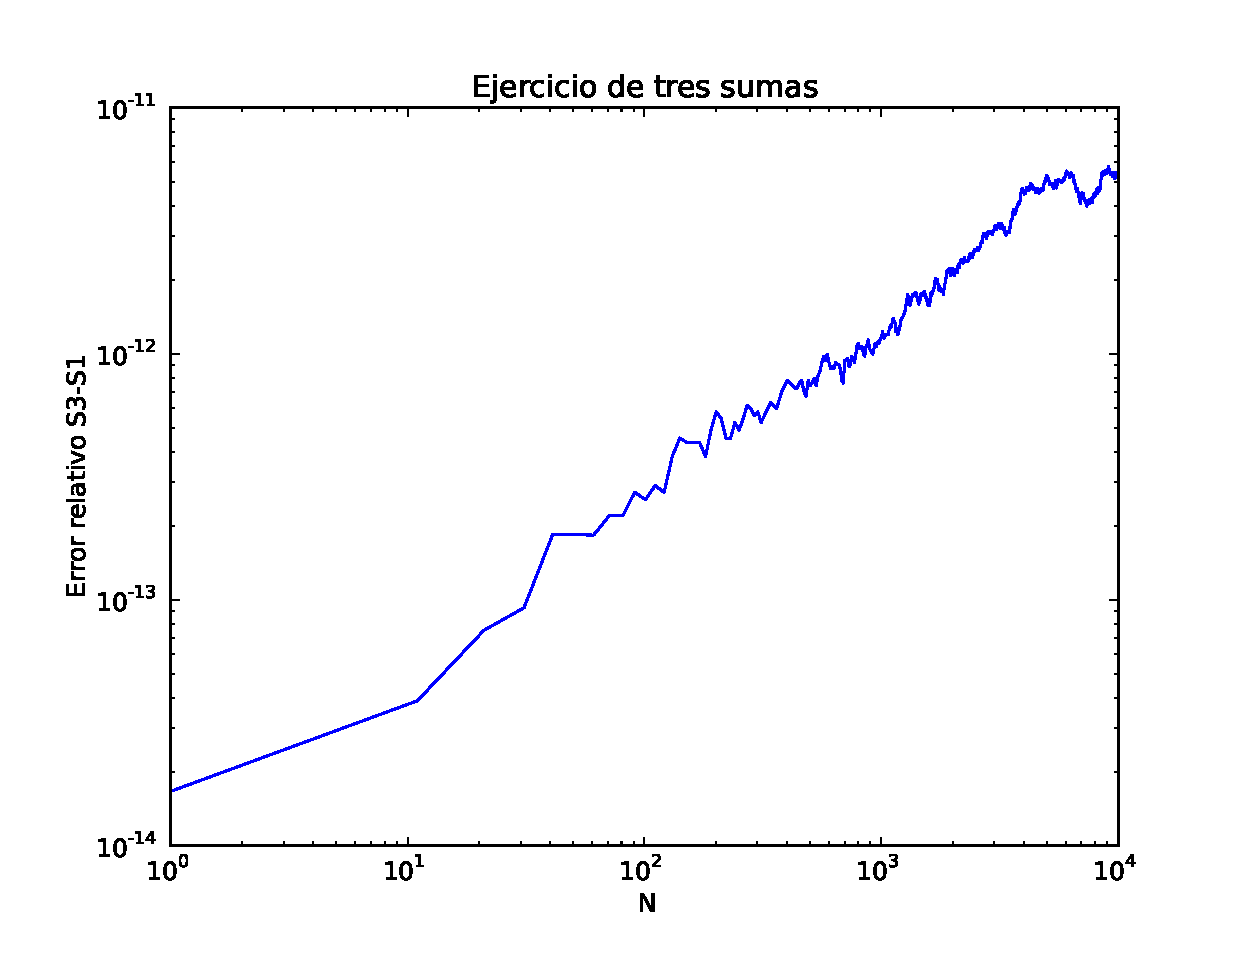
\includegraphics[scale=0.5]{Imagenes/TresSumasS3vsS1.eps} 
\end{figure}
\end{frame}
\begin{frame}
\frametitle{Error relativo entre $S3$ y $S2$}
\begin{figure}
	\centering
	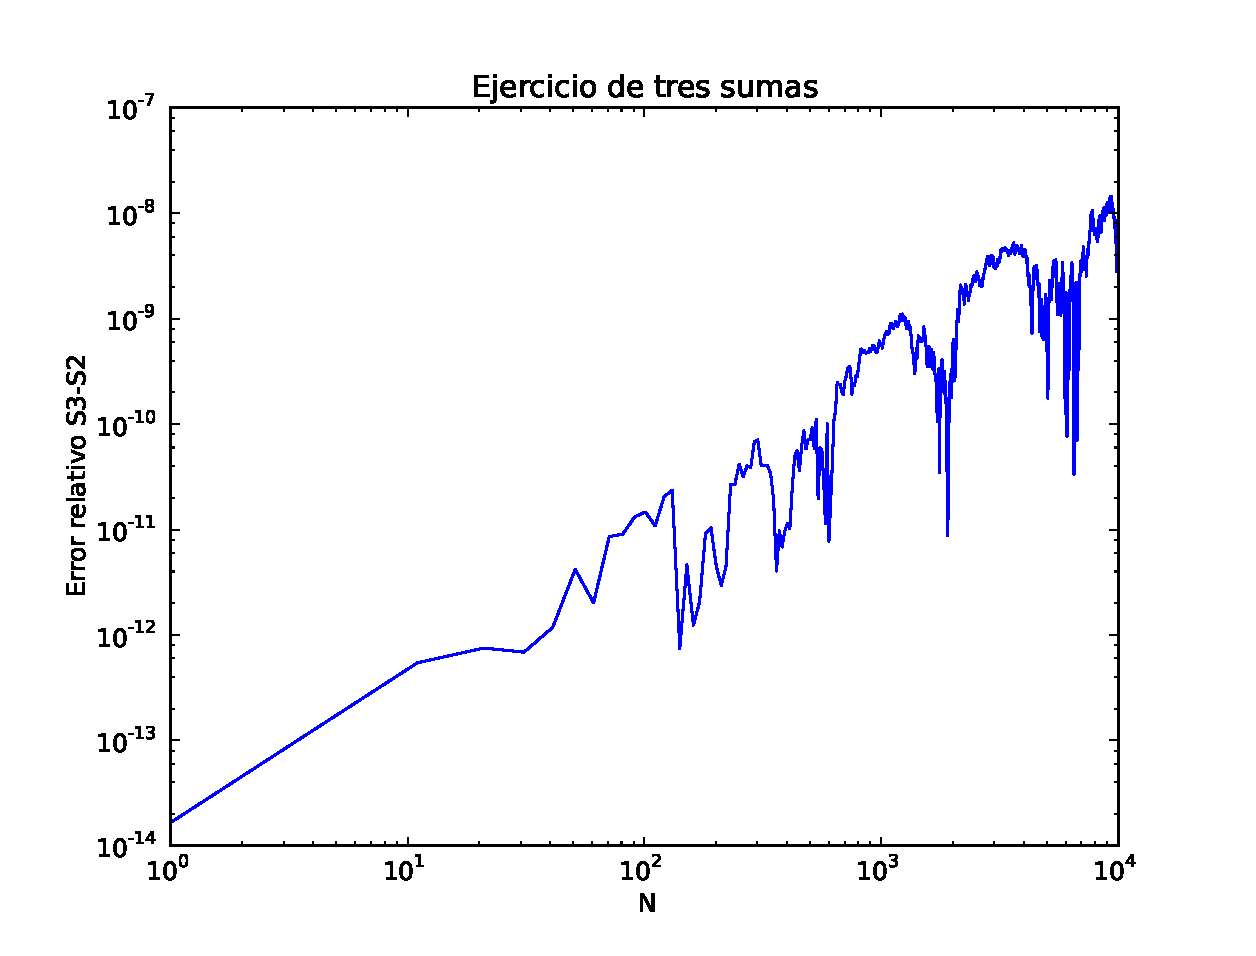
\includegraphics[scale=0.5]{Imagenes/TresSumasS3vsS2.eps} 
\end{figure}
\end{frame}
\begin{frame}
\frametitle{Problema 2}
Aunque tengamos el apoyo de una buena computadora, el cálculo de la suma de una serie requiere reflexión y cuidado.
\\
Considera la serie:
\[S^{(u)} = \sum_{n=1}^{N} \dfrac{1}{n} \]
que será una suma finita mientras $N$ sea finito. Cuando hacemos la suma de manera analítica, no importa si se hace de manera ascendente: desde $n=1,2,3,\ldots,N-1,N$, o descendente: desde $n=N,N-1,N-2,\ldots,3,2,1$
\[S^{(d)} = \sum_{n=N}^{1} \dfrac{1}{n} \]
\end{frame}
\begin{frame}
Sin embargo, debido a los errores por redondeo, cuando calculamos de manera analítica, el valor de las sumas no es el mismo, $S^{(u)} \neq S^{(d)}$
\begin{enumerate}
\item Escribe un programa que calcule $S^{(u)}$ y $S^{(d)}$ como función de  $N$.
\item Grafica (log-log) la diferencia relativa entre la suma relativa contra $N$.
\item Identifica en tu gráfica una región en donde la tendencia es casi lineal, ¿qué representa ésta sección con respecto al error?
\end{enumerate}
\end{frame}
\section{Error por corte/redondeo}
\begin{frame}
Volvamos a nuestro sistema decimal tradicional. Supongamos ahora que los números se pueden representar de la siguiente manera:
\[ fl(x) = \pm (0 . d_{1} d_{2} d_{3} \ldots d_{t} d_{t+1} d_{t+2} \ldots) \times 10^{e} \]
Si la precisión elegida es $t$, entonces ''recortar'' el número definido arriba, pues no podemos representar los $d_{i}$ para $i > t$.
\end{frame}
\begin{frame}[fragile]
En consecuencia, tenemos dos alternativas básicas para efectuar dicho recorte:
\begin{enumerate}[<+->]
\item  \textbf{Corte}: Ignorar los dígitos $d_{i}$ cuando $i > t$
\item \textbf{Redondeo}: Sumar 1 a $d_{t}$ si $d_{t+1}\geq \frac{10}{2}$ e ignorar los restantes $d_{i}$ para $i > t + 1$, o aplicar corte si $d_{t+1} < \frac{10}{2}$
\end{enumerate}
\end{frame}
\begin{frame}
Esto nos permite obtener una cota del error absoluto para ambos casos:
\[ e_{A} = \left\{ \begin{array}{ll}
10^{-t} \times 10^{e} & \mbox{para corte} \\
\dfrac{1}{2} 10^{-t} \times 10^{e} & \mbox{para redondeo}
\end{array} \right. \]
\end{frame}
\begin{frame}
Y como definimos el error absoluto, también podemos definir un límite para el error relativo, que será:
\\
\medskip
\textbf{Corte}:
\[ e_{r} \leq \dfrac{10^{-t} \times 10^{e}}{0.1 \times 10^{e}} = 10^{1-t} \]
\textbf{Redondeo}:
\[e_{r} \leq \dfrac{1}{2}\dfrac{10^{-t} \times 10^{e}}{0.1 \times 10^{e}} = \dfrac{1}{2}10^{1-t}\]
\end{frame}
\begin{frame}
Al valor $10^{1-t}$ lo identificaremos con la letra $\mu$, y resulta ser importante porque nos da
una idea del error relativo que cometemos al utilizar una representación de coma flotante. Suele
denominarse como \textcolor{blue}{unidad de máquina o unidad de redondeo}. El negativo del exponente de $\mu$ suele llamarse también \textit{cantidad de dígitos significativos}.
\end{frame}
\section{Errores de truncamiento}
\begin{frame}
\frametitle{Errores de truncamiento}
Sabemos que este error surge de aproximar procesos continuos mediante procedimientos discretos o
de procesos ''infinitos'' mediante procedimientos ''finitos''.
\\
\medskip
Como ejemplo suele tomarse la diferenciación numérica como forma de aproximar el cálculo de una derivada en un punto (o su equivalente, la integración numérica), en tanto que para el caso de discretización, el ejemplo más es usual es la utilización de métodos iterativos para resolver sistemas de ecuaciones lineales.
\end{frame}
\begin{frame}
En general, el error de truncamiento está asociado al uso de la serie de Taylor para aproximar funciones, de modo que estimar una cota del error no conlleva una dificultad mayor. Sin embargo, en él suelen interactuar el error inherente y/o el de redondeo, con lo que muchas veces su influencia no es bien advertida o es muy reducida. 
\\
\medskip
Veamos un ejemplo clásico: Supongamos que queremos calcular una aproximación de $f'(x_{0})$ para una función continua, pues no es posible obtener la derivada en forma analítica o resulta muy difícil. Por lo tanto, usaremos un entorno del punto $x_{0}$ para calcular $f'(x_{0})$ utilizando solamente $f(x)$.
\end{frame}
\begin{frame}
Para ello nos valdremos de la serie de Taylor. En efecto, para cualquier punto distante $h$ de $x_{0}$ tendremos:
\[ \begin{split}
f(x_{0} + h) = f(x_{0}) + f'(x_{0})h + f''(x_{0}) \dfrac{h^{2}}{2} + \\
{} + f'''(x_{0}) \dfrac{h^{3}}{6} + f^{4}(x_{0}) \dfrac{h^{4}}{24} + \ldots
\end{split} \]
\pause
despejamos $f'(x_{0})$, por tanto
\[ \begin{split} 
f'(x_{0}) = \dfrac{f(x_{0} + h) - f(x_{0})}{h} + \\
- \left[ f''(x_{0}) \dfrac{h^{2}}{2} + f'''(x_{0}) \dfrac{h^{3}}{6} + f^{4}(x_{0}) \dfrac{h^{4}}{24} + \ldots \right] 
\end{split} \]
\end{frame}
\begin{frame}
Si el algoritmo que proponemos para aproximar $f'(x_{0})$ es
\[ f'(x_{0}) = \dfrac{f(x_{0} + h) - f(x_{0})}{h} \]
El error que se comete en la aproximación viene dado por:
\[ \begin{split}
\left[ f'(x_{0}) - \dfrac{f(x_{0} + h) - f(x_{0})}{h} \right] = \\
=  \left[  f''(x_{0}) \dfrac{h^{2}}{2} + f'''(x_{0}) \dfrac{h^{3}}{6} + f^{4}(x_{0}) \dfrac{h^{4}}{24} + \ldots \right] 
\end{split} \]
\end{frame}
\begin{frame}
El término de la derecha es el denominado error de truncamiento, pues es lo que se truncó
a la serie de Taylor para aproximar el valor buscado. 
\\
\medskip
Este error suele asociarse también con la convergencia (o la velocidad de convergencia), que suele representarse como $O(n)$ (generalmente, como $O(h^{n})$, siendo $n$ el parámetro que determina la velocidad o la convergencia. 
\\
\medskip
En nuestro ejemplo, y dado que $h$ generalmente es menor a 1, podemos decir que la aproximación es del tipo:
\[ f'(x_{0}) = \dfrac{f(x_{0} + h) - f(x_{0})}{h} +  O(h)\]
\end{frame}
\begin{frame}
En donde el error que se comete es proporcional a $h$.
\\
\medskip
Se verifica que además están los términos con $h^{2}$, $h^{3}$, etc. pero como $h<1$ se tiene que $h^{2}<<h$, $h^{3} << h^{2}$, etc. por lo que la influencia de éstos es mucho menos y despreciable.
\end{frame}
\begin{frame}
Supongamos por un momento que todas las derivadas $f^{i}(x_{0}) = 0$ para $i \geq 3$. Entonces, tenemos que:
\[ \left[ f'(x_{0}) - \dfrac{f(x_{0} + h) - f(x_{0})}{h} \right] = \dfrac{h}{2} \vert f''(\xi) \vert \]
con $\xi \in [x,x+h]$
\\
\medskip
por lo que, si conociéramos $f''(\xi)$ se podría acotar el error que se está cometiendo por despreciar el término $h/2 f''(x_{0})$
\end{frame}
\begin{frame}
Como ejercicio, apliquemos el algortimo para obtener la derivada en $x_{0}=0.45$, es decir,  $f'(0.45)$ de la función $f(x) = \sin(2 \pi x)$.
\\
\bigskip
Considera el valor exacto de la derivada $f'(0.45) = 2 \pi cos(2 \pi * 0.45) = -5.97566$, toma el valor de $h=0.1$
\end{frame}
\begin{frame}
\frametitle{Construye una tabla}
\begin{center}
\begin{tabular}{l | l | l}
h & $f'(x_{0})$ & Error \\ \hline
$10^{-1}$ & & \\ \hline
$10^{-2}$ & & \\ \hline
$10^{-3}$ & & \\ \hline
$10^{-4}$ & & \\ \hline
$10^{-5}$ & & \\ \hline
$10^{-6}$ & & \\ \hline
\ldots & & \\ \hline
$10^{-16}$ & &
\end{tabular}
\end{center}
\end{frame}
\begin{frame}
\frametitle{Gráfica de la tendencia del error}
\begin{figure}
	\centering
	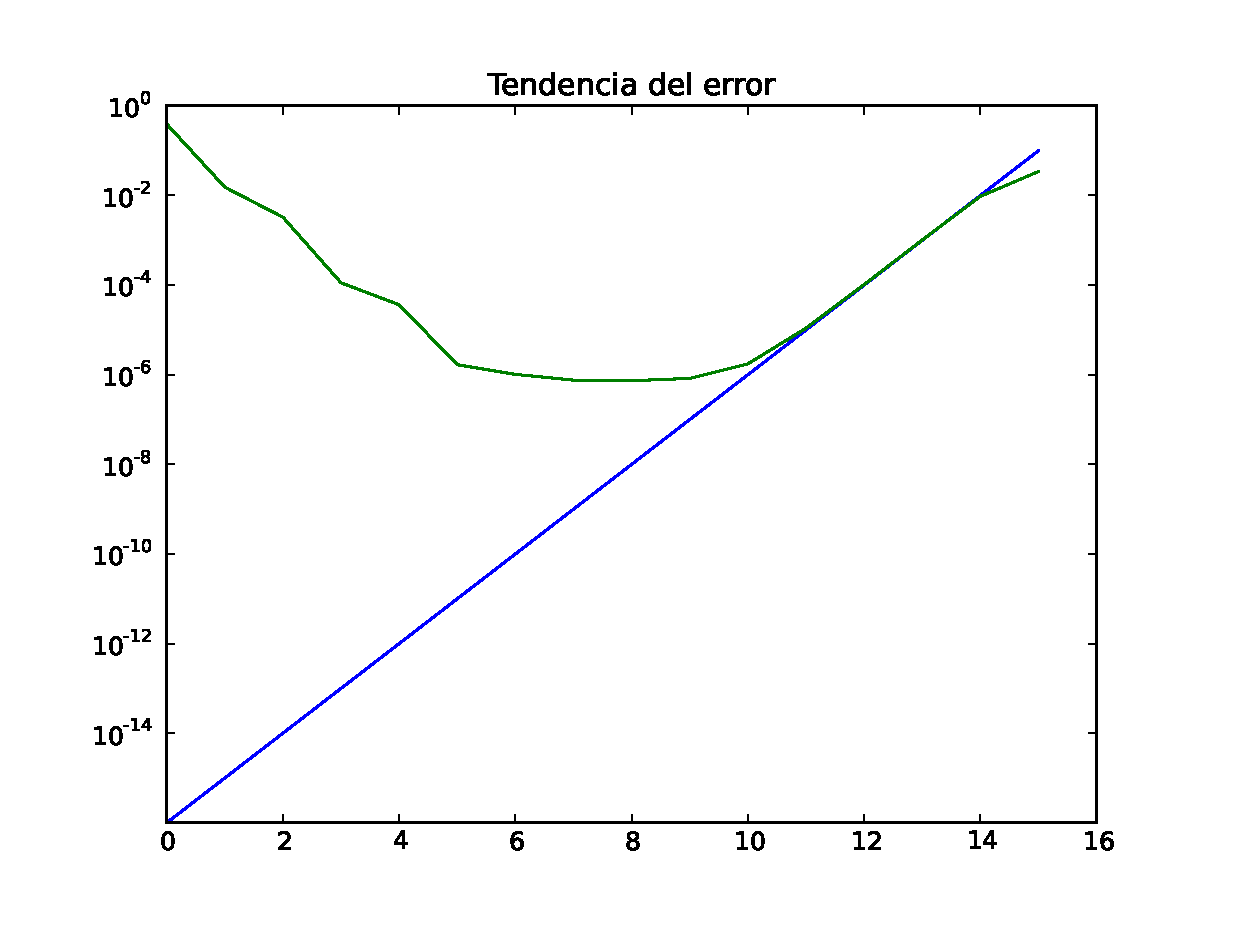
\includegraphics[scale=0.5]{EjercicioTruncamiento.eps} 
\end{figure}
\end{frame}
\begin{frame}
\begin{center}
\begin{tabular}{l | l | l}
h & $f'(x_{0})$ & Error \\ \hline
1e-01 & -6.180340 & 3.425226e-02 \\ \hline
1e-02 & -6.032711 & 9.547183e-03 \\ \hline
1e-03 & -5.981725 & 1.014908e-03 \\ \hline
1e-04 & -5.976274 & 1.027353e-04 \\ \hline
1e-05 & -5.975725 & 1.093152e-05 \\ \hline
1e-06 & -5.975670 & 1.745271e-06 \\ \hline
1e-07 & -5.975665 & 8.269814e-07 \\ \hline
1e-08 & -5.975664 & 7.339002e-07 \\ \hline
1e-09 & -5.975665 & 7.561951e-07 \\ \hline
1e-10 & -5.975666 & 1.016302e-06 \\ \hline
\end{tabular}
\end{center}
\end{frame}
\begin{frame}
\begin{center}
\begin{tabular}{l | l | l}
h & $f'(x_{0})$ & Error \\ \hline
1e-11 & -5.975670 & 1.666570e-05 \\ \hline
1e-12 & -5.975442 & 3.642056e-05 \\ \hline
1e-13 & -5.976331 & 1.122121e-04 \\ \hline
1e-14 & -5.995204 & 3.270657e-03 \\ \hline
1e-15 & -5.884182 & 1.530843e+02 \\ \hline
1e-16 & -8.326673 & 3.934315e+01 \\ \hline
\end{tabular}
\end{center}
\end{frame}
\begin{frame}
Si analizamos en detalle, vemos que la tendencia del error de truncamiento es lineal (en escala logarítmica) pero para $h < 10^{-8}$ el error aumenta y no sigue una ley determinada. Este ''empeoramiento" de la aproximación se debe a la incidencia del error de redondeo, es decir, la unidad de máquina pasa a ser más importante que el error de truncamiento.
\\
\medskip
Es por eso que no siempre el utilizar una ''mejor precisión'' ayuda a mejorar los resultados finales. En este tipo de problemas, es conveniente que el error que domine los cálculos sea el de truncamiento o dediscretización.
\end{frame}
\section{Acumulación del error por redondeo}
\begin{frame}
Desde que se creó la primera computadora, la acumulación del error de redondeo ha sido uno de los ''dolores de cabeza'' de los especialistas, como se puede ver en esta frase:
\\
\medskip
''La extraordinaria rapidez de las actuales computadoras significa que en un problema típico se realizan millones de operaciones con coma (punto) flotante. Esto quiere decir que la acumulación de errores de redondeo puede ser desastrosa''.
\end{frame}
\begin{frame}
En muchas ocasiones la inestabilidad está dada por la incidencia de unos pocos errores de redondeo y no por la acumulación de millones de ellos.
\\
\medskip
Un ejemplo en ese sentido está dado por el algoritmo del ejemplo inicial, en el cual el error está dado por el redondeo de $y_{n-1}$, que se propaga a medida que el valor es cada vez más chico.
\end{frame}
\begin{frame}
\frametitle{Ejercicio}
Calcula el valor de $e$ para $n$ suficientemente grandes, a partir de la su definición:
\[ f(n) = \lim_{n \rightarrow \infty} \left( 1 + \dfrac{1}{n} \right)^{n} \]
\end{frame}
\begin{frame}
Completa la tabla:
\begin{center}
\begin{tabular}{l |l | l}
n & f(n) & $\vert \exp - f(n) \vert$ \\ \hline
$10^{1}$ & & \\ \hline
$10^{2}$ & & \\ \hline
$10^{3}$ & & \\ \hline
\ldots & & \\ \hline
$10^{14}$ & & \\ \hline
$10^{15}$ & & \\ \hline
\end{tabular}
\end{center}
Discute tus resultados!
\end{frame}
\end{document}